\section{Safety in \projname{}}
\label{sec:principle}

% \jinghao{\S\ref{sec:principle}: How to make it safe}

%\begin{itemize}
%    \item goal: expressive and safe (more expressive than and at least as safe
%        as eBPF)
%    \item Current problem of eBPF: the verifier
%    \item Idea: remove the verifier and use a safe language
%    \item the language should be Turing complete and at the same time low-level
%        enough to provide safety features.
%    \item We choose Rust as the implementation language.
%    \item The use of Rust automatically provides eexpresssiveness
%    \item We then show how a safety can be achieved for kernel extensions via
%        language-based safety from Rust.
%    \item how to ensure safety (high-level discussion, no implementation
%        details)
%        \begin{itemize}
%            \item builtin memory/control/type safety
%                \begin{itemize}
%                    \item generic and const-generic functions and slices to
%                        prevent OOB access
%                    \item Safe direct packet access for XDP programs
%                    \item Retired expressiveness kernel helpers (\jinghao{probably does not belong here})
%                \end{itemize}
%            \item RAII (e.g. lock, refcnt)
%            \item exception handling and stack unwinding
%                \begin{itemize}
%                    \item Needed because Rust itself has runtime checks (e.g.
%                        array OOB access)
%                    \item handle exceptional control flow
%                    \item clean up resources to achieve RAII under exceptional
%                        circumstances
%                \end{itemize}
%            \item runtime mechanism to support properties that are
%                (fundamentally) hard to check at compile time
%                \begin{itemize}
%                    \item program termination
%                    \item stack overflow protection
%                \end{itemize}
%        \end{itemize}
%\end{itemize}

% Some small things here and there
%
% - no clone impl for objects returned by RT crate to ensure uniqueness
% - difference between userspace Rust: there are things the compiler cannot see
%   e.g., we cannot have something like Mutex::get_mut in bpf_spinlock to
%   access a value w/o lock using the single-mutable-reference rule


The goal of \projname{} is to provide enhanced usability for kernel extensions,
    while ensuring safety of the extension programs.
In particular, we aim to make \projname{} more usable than eBPF and as safe.
As discussed in \S\ref{sec:motivation}, the current problem of usability of
    eBPF is the large \gap{}. % between the programer, who works on
    % high-level languages, and the verifier, which operates on compiled bytecode.
% Our insight is that both the needed expressiveness and safety can be obtained
%     from a safe programming language without the verifier.
Our insight is that by using a safe, high-level language that directly
    implements the required safety properties of kernel extensions, the need
    of the extra verification layer can be dropped, and thereby closing the
    \gap{}.
\mvle{not completely true tho since we need the runtime part for termination}

% Specifically, the language should have the following properties:
% \begin{itemize}
%     \item \textbf{Turing-complete}: This helps to satisfy the expressiveness
%         requirement.
%     \item \textbf{Safe}: The language should not be as permissive and
%         error-prone as unsafe languages like C.
%     \item \textbf{Low-level}: Being low-level helps the programs to better
%         model low-level kernel semantics and simplifies infrastructure needed
%         to support it.
% \end{itemize}

% \djw{background on Rust moves here}
% Need to talk about:
% - Language-based safety no undefined behavior in Rust.
% - Safe/unsafe Rust.
% - Popularity (also embraced by kernel)

\projname{} chooses Rust as the safe language for extension programs.
Rust is a system programming language that aims to provide
    \emph{language-based} safety, which promises programs to be free of
    \emph{undefined behaviors}.
The compiler both performs static analysis (e.g., lifetime and ownership
    models) and inserts dynamic checks (e.g. array bounds checks) in
    Rust programs to fulfill its safety promises.
To facilitate low-level code that may be hard to fit into its safety model (e.g.
    FFI calls), the language also provides \emph{unsafe} Rust, which is more
    permissive and provides a weaker safety guarantee, as opposed to
    \emph{safe} Rust.
Utilization of the language-based safety of Rust under kernel contexts has been
    explored by previous works~\cite{redleaf,theseus}, and is also incorporated
    into the Linux kernel~\cite{rust-for-linux-lwn}.
% This is because Rust happens to provide the desired properties -- its
%     language-based safety can be leveraged for safe kernel extensions without a
%     verifier.
In \projname{}, Rust provides either the desired properties directly or
    essential building blocks to ensure the important safety properties for
    kernel extensions (\S\ref{sec:background}).
% Here, we list the important safety properties
% (\jinghao{may need to move to \S\ref{sec:background}})
% \begin{itemize}
%     \item Memory safety
%     \item Type safety
%     \item Safe resource management
%     \item Exception-based runtime safety
%     \item Stack safety
%     \item Program termination
% \end{itemize}

% \jinghao{The runtime exception handling is not necessarily an independent one,
% it actually covers some of the type safety (arrays and slices does runtime
% checks that may trigger exceptions)}
\begin{figure}
    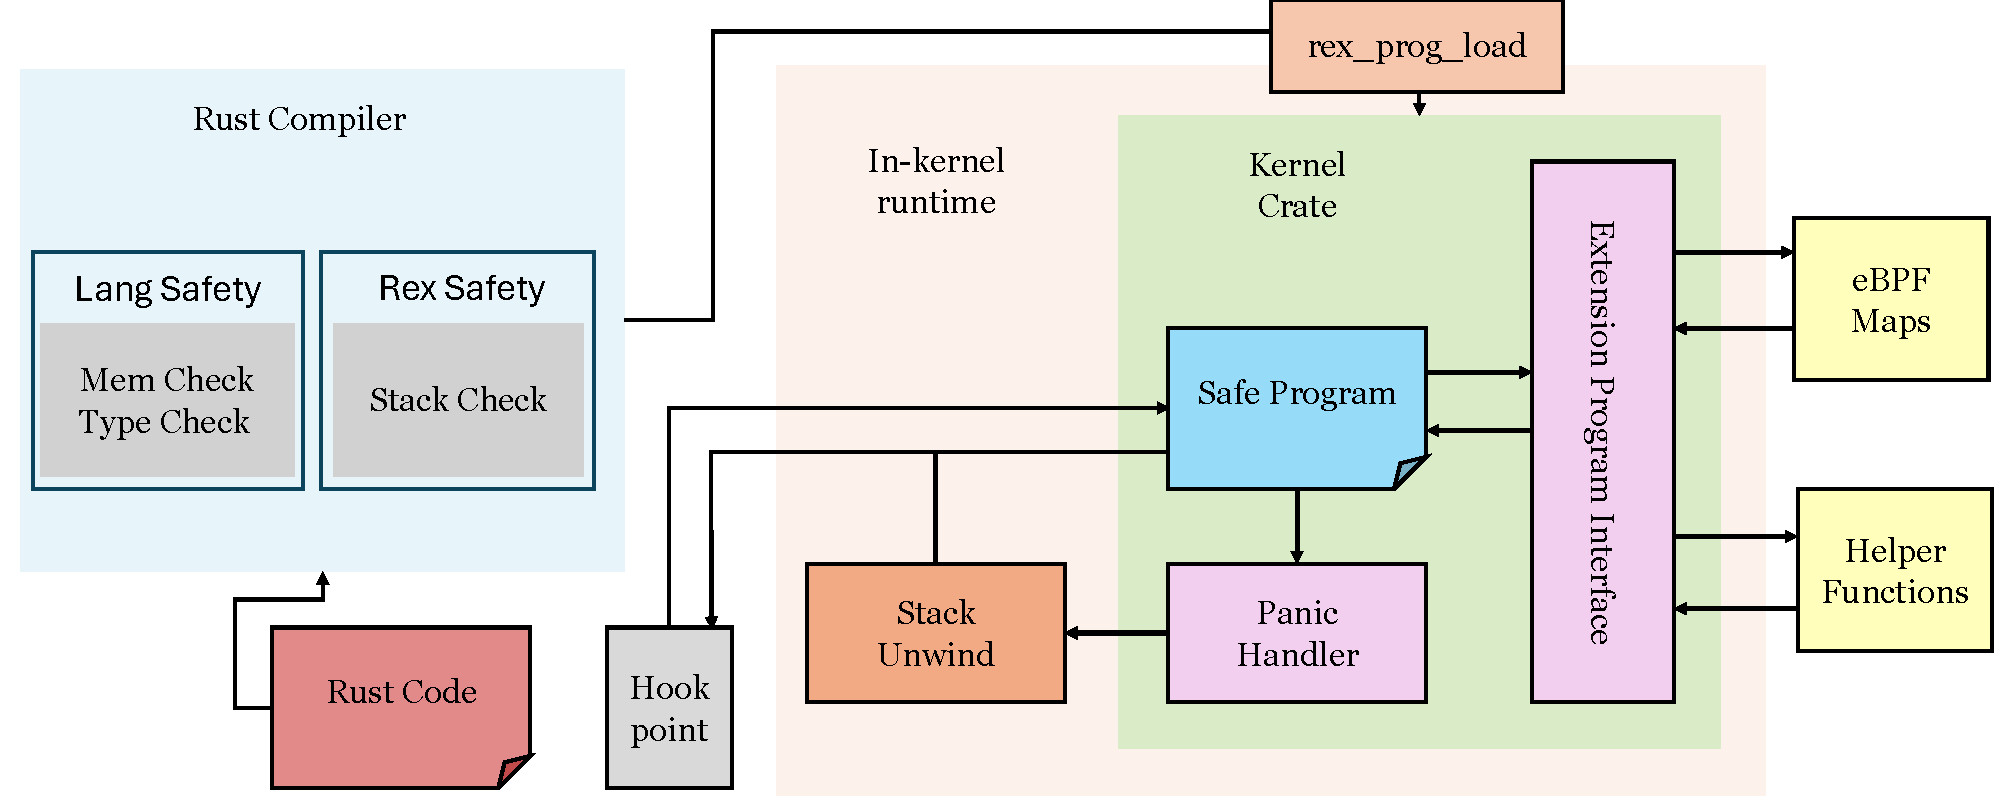
\includegraphics[width=1.0\linewidth]{figs/overview.pdf}
    \centering
    \vspace{-10pt}
    \caption{Overview of \projname{}}
    \label{fig:rex-overview}
    \vspace{-10pt}
\end{figure}

We now discuss how the language-based safety from Rust can be applied to the
    context of kernel extensions to provide a safe programming interface.
% While the use of Rust automatically provides expressiveness (as it is
%     Turing-complete), it does not supply the safety out-of-box, and the use of
%     Rust, especially unsafe Rust, can still exhibit undesired behaviors.
% We require all extension programs to be implemented \emph{only} in safe Rust.
% On top of that, we discuss how the safety properties from Rust can be leveraged
%     and applied to the context of kernel extensions to provide a safe
%     programming interface.
Figure~\ref{fig:rex-overview} provides an overview of the \projname{} framework.
The extension program is written strictly in \emph{safe} Rust.
It is compiled by the Rust compiler, which not only ensures safety properties
    in Rust but also runs a \projname{}-specific pass for kernel stack safety.
The program interacts with the kernel through a program interface implemented
    by the \projname{} \emph{kernel crate}.
The kernel crate contains a mixture of unsafe Rust code due to its role as a
    bridge between the extension program, which is expected to be checked for
    safety, and the unsafe but trusted kernel code.
It also provides a custom Rust panic handler to support panic-based runtime
    safety checks in Rust.
The program links with the kernel crate at compile time and runs in a
    light-weight runtime environment implemented in the kernel, which provides
    program termination and stack unwinding support.

\subsection{Memory safety}
\label{principle:memsafety}
Generally, kernel extensions are not allowed to access kernel memory.
However, there are frequent cases that an extension program needs to work on a
    shared buffer of data or a specific struct, and exchange data with the
    kernel.
% These regions of memory are accessed by both the program via helper functions
%     and the kernel.
% Rust provides powerful primitives that help to validate the memory is
%     accessed correctly.
There are usually two common patterns on how the memory is accessed, differing
    by the owner of the memory: 1) Memory owned by the extension program (e.g.,
    an on-stack buffer) is sent to the kernel through the helper function
    interface. 2) Memory owned by the kernel (e.g., an in-kernel struct) is
    accessed from the extension program. % direct packet access, map data ptr

In the first case, the extension program may allocate some memory on the stack
    and send it to the kernel for processing (e.g., asking kernel to fill a
    stack buffer with some data).
An unsafe memory access, for example, an out-of-bounds write to the on-stack
    buffer, could result in corruption of stack data and possibly trigger a
    kernel crash if the return address is overwritten to a non-present page.

For eBPF, the verifier validates the memory region with the size to make sure
    that both the kernel and the program do not make erroneous accesses.
For the memory buffers sent to the kernel through the helper function interface,
    the corresponding size is also sent as an argument to the helper.
The verifier, at program load time, checks to ensure that the size is exactly
    that of the memory buffer.
Then, at runtime, the kernel can operate on the buffer with the knowledge of
    its bounds, thereby avoid unsafe memory accesses.

In \projname{}, the strict type system of Rust already protects the program
    from making an unsafe access.
\projname{} leverages the generic programming feature of Rust to ensure the
    size sent through the helper function interface is always valid.
% In order to make sure that the size sent to the kernel is always correct, which
%     is vital for the correctness of memory access from the kernel, we leverage
%     the generic programming support of Rust.
For kernel helper functions that take in a
    program-supplied pointer and size, the \projname{} kernel crate creates an
    adaptor interface that parametrizes the type of the pointer as a generic
    type parameter.
The interface queries the size of the generic type from the compiler
    and invokes the kernel interface with this size as the argument.
Since Rust employs monomorphization~\cite{rustc-monomorphize}, the concrete
    type and its size is resolved at compile time, adding no runtime overhead.
In this way, the size is guaranteed to match the type statically and the
    kernel will never make an out-of-bound access.
This can work for not only scalar types, but array types as well: Rust
    also supports ``const generics'' that allows a constant to be used as a
    generic parameter, which can be used to encode the length of arrays.

In the second case, the kernel may provide the user program a pointer to
    kernel memory to perform direct access (e.g., access through eBPF map value
    pointers and packet pointers).
The user programs must not make an out-of-bound memory access for this
    kernel-owned region of memory, as doing so risks corrupting kernel data.

In eBPF, for accesses on pointers with a static size, e.g. map value pointers,
    as maps store the size of its value types, the verifier can independently
    verify the validity.
For pointers without a static size like packet data pointers, the verifier
    enforces programs to explicitly check for memory
    boundaries and to not make out-of-bound accesses.

In \projname{}, pointers with a static size are handled through the Rust type
    system, as the
    kernel map interface of \projname{} encodes the key and value types through
    generics.
The type system therefore forces the pointer to be a safe Rust reference of
    the particular type.
Pointers referring to a memory region without a static size are generally
    dynamic-sized buffers.
The \projname{} kernel crate abstracts such pointers into a Rust \emph{slice}
    with dynamic size.
Rust slice provides runtime bounds checks (\S\ref{principle:eh}), which allows
    the check to happen automatically without explicit handling from the
    extension program.

\subsection{Extended type safety}
Kernel extensions may contain certain paradigms that are beyond the safe
    type system of Rust.
One challenge is to allow extension programs to safely reinterpret the stream
    of bytes into useful data.
Such cases are notably found in networking use cases, where a program may need
    to extract the Ethernet header from a byte buffer in the packet.
Safety of these transformations is hard to reason about because they
    inevitably involve unsafe type casting.
% For example, a XDP program using direct packet access might need to extract
%     the ethernet header information from the bytes in the packet.

Currently, eBPF allows the program to freely interpret the packet data into
    other data types via pointer casting.
The verifier checks the casting and ensures that 1) the program does not make a
    pointer from scalar values and 2) the new type fits within the memory
    boundaries.

\projname{} agrees with the verifier that as long as the above two properties
    hold, the reinterpreting cast (dubbed ``transmute'' in Rust) is safe to
    perform.
It therefore extends the type safety of Rust to cover such cases.
% In the case of Rust, the reinterpret cast (dubbed ``transmute'' in Rust) is an
%     unsafe operation, particularly because Rust does not prevent making
%     pointers from scalar values.
To allow extension programs to still safely reinterpret the bytes into useful
    data types, \projname{} defines a group of primitive scalar types that are
    considered safe as targets for casting.
\projname{} requires the target type of casting to be of either the safe types
    or a structure type in which all the members are of the safe types.
The safe types are specified by implementing the \texttt{Rex::SafeTransmute}
    trait, which is only implementable by code within the kernel crate.

We use the \emph{proc-macro} feature of Rust to enforce this constraint at
    compile time.
Like conventional C macros, proc-macros performs transformation on the program,
    albeit on the abstract syntax tree level.
Our proc-macro, when applied on a structure type, generates code that tries
    to treat each field of the structure as an instance of
    \texttt{Rex::SafeTransmute} using Rust trait bounds, followed by the actual
    transmute operation to perform the unsafe cast.
If one of the fields in the structure does not implement
    \texttt{Rex::SafeTransmute}, the Rust compiler will issue a compile error.
At the same time, if the program tries to directly transmute the bytes into a
    structure without using the proc-macro, the compiler will also emit an
    error because transmute belongs to unsafe Rust, which is forbidden in
    \projname{} programs.
Since proc-macro transformations happen after the linting of unsafe operations,
    the transmute code generated by the proc-macro will not be rejected and,
    therefore, allows programs to perform transmutes in a safe, and controlled
    way.
\jinghao{Shall we remove this sentence, people may ask whether programs can
use proc-macros to get around the safe Rust requirement}

\subsection{Safe resource management}
%Executing in the kernel,
Extension programs must also acquire and release
    resources properly under kernel context.
Some kernel helper functions return kernel resources that require
    explicit release after use through corresponding helper function calls.
Failing to do so will result in leakage of kernel resources such as reference
    counts and acquired spinlocks.
% In eBPF, some kernel helper functions returns kernel resources that requires
%     explicit release after use (e.g., reference counts of kernel objects,
%     locks).

In these situations, the eBPF verifier checks and ensures that the resource is
    released on all possible code paths to prevent leaking kernel resources.

\projname{} leverages the resource-acquisition-is-initialization
    (RAII)~\cite{rust-raii} pattern of Rust: for each kernel resource that
    extension programs need, \projname{} creates an RAII wrapper type that ties
    the resource with the lifetime of the wrapper object.
For example, when the program obtains a spinlock from the kernel, the
    \projname{} kernel crate constructs and returns a \emph{lock guard}.
The lock guard implements the RAII semantics through the
    \texttt{drop}~\cite{rust-drop} trait in
    Rust, which defines the operation to perform when an object is destroyed.
In the case of lock guard, its \texttt{drop} handler releases the lock.
The program does not need to explicitly release the lock or drop the lock
    guard, instead, the compiler inserts an implicit \texttt{drop} at the end
    of the current scope. This effectively releases the lock when the lock
    guard goes out of scope.

\subsection{Runtime exception handling}
\label{principle:eh}
While the compiler contributes a lot to the safety of Rust, unlike eBPF, many
    safety checks happen at runtime in the form of exceptions (i.e., Rust
    panics).
In userspace, Rust uses the Itanium exception handling ABI~\cite{itanium-abi}.
When an exception is triggered, the control flow is transferred to the Rust
    panic handler in its standard library, which in turn calls into the unwind
    library to perform stack unwinding and resource cleanups for each stack
    frame.
However, the Itanium ABI is complex and not suitable for kernel extensions,
    making exception handling a challenge in \projname{} extension programs:
\begin{itemize}
%     \item The Itanium ABI-based exception handling is too complicated, as the
%         userspace unwind libraries are not direcly usable.
    \item Failures during unwinding, which are permissible in userspace, cannot
        be tolerated in kernel space, as incomplete cleanup means leaking
        kernel resources.
    \item ABI-based unwinding typically requires dynamic allocation, which
        creates challenges for extensions in interrupt contexts, in which an
        allocator may not be available~\cite{bpf-mempool-lwn}. \jinghao{I'm
        thinking about removing this one since bpf now has an allocator.}
    \item Unwinding generally executes destructors for all existing objects on
        the stack, but executing untrusted, user-defined destructors (via the
        \texttt{\small Drop} trait in Rust) is not safe.
\end{itemize}

\begin{figure}
    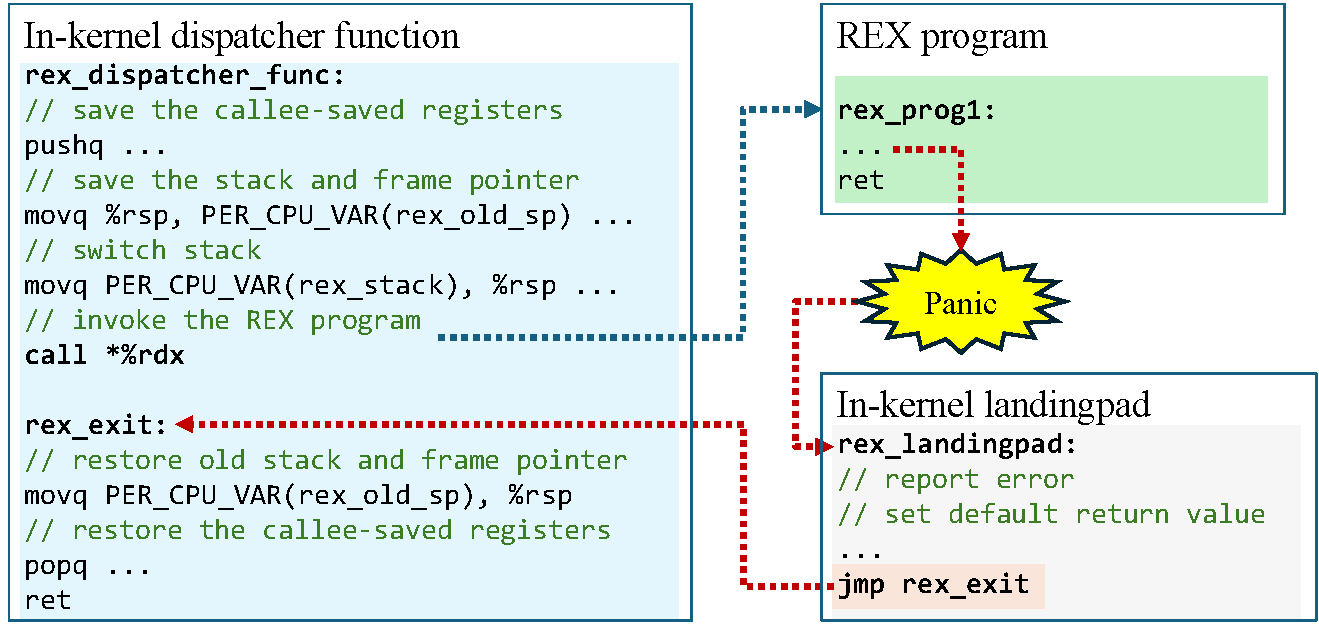
\includegraphics[width=1.0\linewidth]{figs/exception_handling.pdf}
    \centering
    \vspace{-10pt}
    \caption{Exception handling control flow in \projname{}}
    \label{fig:eh-overview}
    \vspace{-10pt}
\end{figure}

Our exception handling framework consists of two components: 1) graceful exit
    upon exceptions that resets the current context and 2) resource cleanup to
    ensure release of kernel resources like reference counts and locks.

\para{Graceful exit:}
To support a graceful exit from an exception, \projname{} implements a small
    runtime (as shown in Figure~\ref{fig:eh-overview}) in the kernel that
    contains a program dispatcher, a panic handler, and a landingpad function.
The dispatcher function takes the same duty of executing the extension program
    as the existing eBPF dispatcher.
It saves the old stack and frame pointer of the current context into per-CPU
    memory before switching to the dedicated program stack
    (\S\ref{principle:stack}) and calling into the program.
If the program exits normally, without triggering an exception, it would
    return to the dispatcher, which switches the stack back.
Under exceptional cases where a Rust panic is triggered, the panic handler will
    release the kernel resources currently allocated by the program, and
    transfer the control flow to the in-kernel landingpad function to print
    debug information related to the exception (e.g., exception message) to the
    kernel ring buffer.
Then, the landingpad function redirects the control flow to a pre-defined label
    in the middle of the dispatcher function, where it restores the old value
    of the stack and frame pointer from the per-CPU storage.
This effectively unwinds the stack and resets the context as if the extension
    program returned successfully.
% We implement the program dispatcher function with panic handling in the kernel
%     in 28 lines of x86 assembly code.

\para{Resource cleanup:}
Light-weight mechanisms can be effective for resource cleanup in \projname{}.
Our insight for resource cleanup is that the extension program can only obtain
    resources by explicitly issuing helper function calls and therefore only
    these resources need to be released.
For these helper function calls, we record the allocated kernel resource during
    execution into a statically defined per-CPU buffer.
Our current implementation can support at most 64
    instances of kernel resources during a single run.
Upon a panic, the panic handler will take the responsibility to correctly
    handle the release of kernel resources, which involves traversing the
    per-CPU buffer and performs cleanup for each of the recorded resources.

% \jinghao{It seems that nesting should be put somewhere, due to the fact that
% these per-CPU tricks depend on no-nesting.}

We implement the cleanup code as part of the \projname{} kernel crate, as it
    is the core component responsible for coordinating helper function calls
    that obtain kernel resources.
% In this way, the resource cleanup is completely transparent to the extension
%     programs, adding no additional programming burden like the Itanium ABI.
The other reason for implementing cleanup mechanism inside the kernel crate is
    safety, because such code maybe called upon panic, it must not trigger yet
    another Rust panic and causes panic handling to fail.
Therefore, \projname{} does not execute user-supplied \texttt{drop} handlers
    upon panic, as they are not guarranteed to be safe during panic handling
    context and programs cannot allocate resources without helper function
    calls.

\subsection{Kernel stack safe guarding}
\label{principle:stack}
One unique safety requirement that kernel extension programs face is the
    usage of kernel stack.
Unlike userspace programs, where the stack grows on demand and has a large
    maximum size,
    the stack in kernel space is fix-sized (4 pages on x86-64) and limited.
Overflowing the kernel stack may result in memory corruptions or kernel panics.

The eBPF verifier handles stack safety by keeping track of the stack size
    throughout its symbolic execution process.
However, the verification of the stack usage does not always yield the correct
    result -- in particular, the verifier has been shown to fail to track stack
    usage across indirect tail calls~\cite{ebpf-stackoverflow}.

Our observation is that the enforcement of stack safety can be easily performed
    at compile time if the extension program does not have indirect or
    recursive calls, and conversely, it is easier to perform such check at
    runtime when the program does employ indirect or recursive calls.
\projname{} therefore takes a hybrid approach in ensuring stack safety that
    utilizes static checks for programs without indirect or recursive calls,
    and dynamic, runtime checks for programs make use of these function calls.
For each program being compiled, the \projname{}-specific pass in the compiler
    will check whether it involves indirect or recursive calls.
When the extension program contains only direct, non-recursive function calls,
    its total stack usage can be calculated by traversing its static callgraph
    and sum up the size of each call frame.
If the total stack usage of the program exceeds total amount of stack
    available, the \projname{} compiler pass will generate an error and reject
    the program.

On the other hand, programs with indirect or recursive calls are hard to check
    for stack usage statically, as is the case in the eBPF verifier.
In these cases, \projname{} performs runtime checks to limit the stack usage of
    programs.
The \projname{} compiler pass first ensures each function in the program takes
    less than one page (4K) of stack.
Then, before each function call in the extension program, the \projname{}
    compiler pass inserts a call to \texttt{\_\_rex\_check\_stack} function.
\texttt{\_\_rex\_check\_stack} is provided by the kernel crate and checks the
    current stack depth of the program, if the stack usage exceeds the
    threshold, it will trigger a Rust panic and effectively terminate the
    program (\S\ref{principle:eh}).

In order for the \texttt{\_\_rex\_check\_stack} function to have more control
    on the stack usage of the program and also support programs with slightly
    large stack usage, \projname{} implements a dedicated kernel stack for the
    extension programs.
The dedicated kernel stacks are allocated per-CPU and virtually mapped during
    kernel boot time with the same size as the kernel IRQ and task stacks.
In the dispatcher function (Figure~\ref{fig:eh-overview}), before calling into
    the \projname{} program, the stack and frame pointers of the current
    context are saved.
The dispatcher function then sets the stack and frame pointer registers to the
    top of the dedicated stack and invokes the program.
Upon program exit, the original stack and frame pointers are restored, no
    matter whether a exception is triggered during program execution.

\projname{} defines the stack usage threshold to be two pages less than the
    total stack available.
This design choice is based on two considerations.
First, kernel helper functions are not visible at program compile time but they
    also account for stack usage during program execution.
Leaving extra spaces accomodates kernel helper functions and we believe two
    pages of stack is a reasonable limit for kernel helper functions.
Second, since the stack usage of each function in the program is limited to
    1 page of stack, in the worse case the remaining stack space is at least
    one page when \texttt{\_\_rex\_check\_stack} triggers a Rust panic.
This worse case guarantee leaves enough space for the panic handling and stack
    unwinding routines.
Such a dynamic mechanism allows \projname{} to achieve better stack-safety than
    eBPF, which only relies on static verification.

\subsection{Bounded program runtime}
\label{principle:termination}
% A bounded program runtime is important for kernel safety
%   - a potentially long running program can hold the CPU and cause kernel
%     lockups
% eBPF handles this by imposing verification limit (ref S3)
%   (Side note:
%    First, this is really ``bounded runtime'' rather than termination, because
%      a long-running program that eventually terminate is almost equally bad
%    Why would programs ever hit that limit if they are supposed to have an
%    acceptable runtime? Is it because of these two reasons:
%      1. The verifier misses some key information that can reduce the search
%         space drastically, as is the case of unbounded loops?
%      2. If the program is meant to execute that many instructions (current
%         limit is 1M), is it because the current limitation is still too small
%         or is it that the program is badly implemented and actually runs
%         longer? (Also, how long would 1M eBPF instructions run with
%         interpretation and JIT?)
%   )
%   - A program that goes over the limit gets rejected, no matter whether it will
%     actually run long
%   - creates usability issues
%   - previous works has also demonstrated ways of creating long running programs
%     without going over the limit (cite raj-lpc and jinghao-hotos)
%
% Given the ineffectiveness and usability issues associated with the static
%   verification approach, Rex uses a dynamic mechanism that interrupts and
%   terminates programs.
% When a program goes over its time limit, it will be terminated.
% The dynamic termination in Rex limits the runtime of the program through a
%   timer.
% When the timer expires, it issues an IPI to the CPU the program is running.
% The IPI effectively suspends the program and saves its registers to the stack.
% Inside the IPI handler, the timeout handler for Rex is executed, which
%   modifies the instruction pointer stored on the stack to the panic handler
%   of rex programs.
% After returning from the IPI the program will be executing the panic handler
%   to gracefully exit.
%
% Challenge: no termination in helpers/panic handlers
%
% We use a per-CPU flag to solve this

Having a bounded runtime for extension programs is critical for safety of the
    kernel.
A long-running extension program could hold the processor for a long time and
    cause kernel lockups.

eBPF addresses potentially long-running programs by imposing a static limit on
    the number of instructions the verifier would go through.
A program that goes over the instruction limit will be rejected by the
    verifier, no matter whether the program will actually run for a long time.
This techinque creates many false-positives and is one of the main sources of
    the usability issues in eBPF, as discussed in
    \S\ref{motivation:restructure}.
Previous works~\cite{ebpf-termination,untenableVerification} have also
    demonstrated creation of long-running eBPF programs without going over the
    verification limits, further weakening the runtime guarrantee from the
    verifier.

Given the usability issues and ineffectiveness associated with the static
    verification approach, \projname{} employs a dynamic mechanism that
    interrupts and terminates long-running programs at runtime.
% \projname{} supports dynamic program termination through an additional API in the kernel's
% BPF syscall interface.
The dynamic termination in \projname{} limits the runtime of the program
    through a timer.
When the timer expires, it issues an inter-processor interrupt (IPI) to the CPU
    the program is running on.
This IPI effectively suspends the program and pushes its registers onto the
    stack.
Inside the IPI handler, the timeout termination handler of \projname{} is
    executed, which modifies the saved instruction pointer register to the
    panic handler of the program.
After returning from the IPI, the program will be executing the panic handler,
    which cleans up kernel resources allocated by the program and gracefully
    exits the program.
% The termination logic uses the Linux kernel's Inter-Process Interrupt (IPI) mechanism
% to raise an interrupt on the target \projname{} program's CPU.
% Depending on the use-case, the IPI can be triggered by an operator or a timer within the system
% that is configured to notify when the \projname{} exceeds a certain runtime threshold.
% Note that we are assuming the availability of a free CPU for an operator to be able to invoke
% an IPI.
% In uniprocessor machines, where the only CPU will be busy running the extension, the operator
% won't be able to issue termination request and has to rely on installing timers.
% We find this limitation acceptable due to the current cloud infrastructure predominantly being SMP.

% To safely terminate a \projname{} extension, we need to ensure the following :
One challenge involved in terminating a \projname{} program safely is that a
    program should never be terminated while executing the kernel helper
    function or the panic handler, as doing so disrupts internal bookkeeping of
    the kernel (e.g. acquired resources) and safe exception handling process of
    \projname{}.
To address this challenge, \projname{} defers termination when the program is
    running kernel helper functions, and does not attempt to terminate if the
    program is already in the panic handler on the exit path.
% \begin{enumerate}
%     \item A \projname{} program should never be terminated while executing a
%         kernel helper function or the panic handler, as doing so disrupts
%         internal bookkeeping of the kernel (e.g. acquired resources) and safe
%         exception handling process of \projname{}.
%         This is neccesary to ensure kernel objects acquired during a helper call
%         are freed.
%     \item Kernel resources allocated within the extension program cannot be
%         left unreleased and cause resource leaks.
% \end{enumerate}

% The raised interrupt handler first detaches the \projname{} program from its hookpoint to prevent
% further invocation.
% The handler then changes the saved registers(in the interrupt stack) from the \projname{} context
%  to point to the \projname{} panic handler(section \ref{principle:eh}).
% The CPU returns the execution to the panic handler which performs the cleanup of
% any kernel objects that were live at the time of termination.
% To address the case when the target \projname{} program could be inside a helper/panic handler,
% \begin{figure}
%     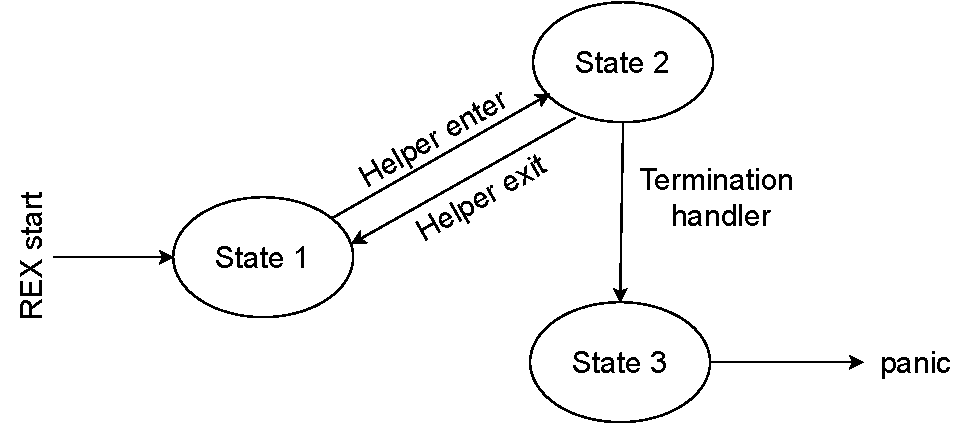
\includegraphics[width=1.0\linewidth]{figs/BPF_termination_state_diagram.pdf}
%     \centering
%     %\vspace{-10pt}
%     \caption{Termination state diagram for \projname{} extensions}
%     \label{fig:rex-termination}
%     %\vspace{-30pt}
% \end{figure}

\projname{} uses a per-CPU tristate flag to keep track the state that the
    extension program is currently in. % (Figure~\ref{fig:rex-termination}).
The states are: 1) executing extension code, 2) executing kernel helpers or
    panic handlers, and 3) termination requested.
Every helper invocation changes the state from state 1) to state 2).
When excuting the timeout termination handler, if the flag is at state 2),
    which indicates the program is in a context that cannot be safely
    terminated, the termination handler modifies it to state 3) without
    setting the instruction pointer.
On a helper function return, the flag is checked and if it is set to state 3),
    the panic handler is called to gracefully exit the program.
% This mechanism is used to defer a panic invocation until the end of a helper execution.
% \jinghao{Shall we have a state diagram?}
